\documentclass{article} % For LaTeX2e
\usepackage{iclr2022_conference,times}
\usepackage{graphicx}
\usepackage{booktabs}
\usepackage{multirow}
\usepackage{amsmath}
% Optional math commands from https://github.com/goodfeli/dlbook_notation.
\input{math_commands.tex}

%######## APS360: Uncomment your submission name
%\newcommand{\apsname}{Project Proposal}
%\newcommand{\apsname}{Progress Report}
\newcommand{\apsname}{Final Report}

%######## APS360: Put your Group Number here
\newcommand{\gpnumber}{42}

\usepackage{hyperref}
\usepackage{url}
\usepackage{graphicx}
\usepackage{tabularx}
\usepackage{geometry}


%######## APS360: Put your project Title here
\title{SynthLens: An AI-Generated Image Detector and Classifier}


%######## APS360: Put your names, student IDs and Emails here
\author{Vedansh Mehta  \\
Student\# 1008973577 \\
\texttt{vedansh.mehta@mail.utoronto.ca} \\
\And
Nathan Shreve  \\
Student\# 1004404487 \\
\texttt{n.shreve@mail.utoronto.ca} \\
\AND
William Wen  \\
Student\# 1007956650 \\
\texttt{jwilliam.wen@mail.utoronto.ca} \\
\And
Paul Zhao \\
Student\# 1009052276 \\
\texttt{paul.zhao@mail.utoronto.ca} \\
\AND
}

% The \author macro works with any number of authors. There are two commands
% used to separate the names and addresses of multiple authors: \And and \AND.
%
% Using \And between authors leaves it to \LaTeX{} to determine where to break
% the lines. Using \AND forces a linebreak at that point. So, if \LaTeX{}
% puts 3 of 4 authors names on the first line, and the last on the second
% line, try using \AND instead of \And before the third author name.

\newcommand{\fix}{\marginpar{FIX}}
\newcommand{\new}{\marginpar{NEW}}

\iclrfinalcopy 
%######## APS360: Document starts here
\begin{document}


\maketitle

\begin{abstract}
    This template should be used for all your project related reports in APS360 course. -- Write an abstract for your project here. Please review the \textbf{ First Course Tutorial} for a quick start
    %######## APS360: Do not change the next line. This shows your Main body page count.
    ----Total Pages: \pageref{last_page}
\end{abstract}



\section{Introduction}



\section{Illustration / Figure}

\begin{figure}[h]
    \begin{center}
        \includegraphics[scale=0.45]{figs/EffiVit.pdf}
    \end{center}
    \caption{Final Architecture}
    \label{fig:EffVit Architecture}
\end{figure}

\section{Background \& Related Work}

Image synthesis is the process wherein an artificial image is generated by a computer from an input prompt, which may be text or some other form of media. This field exploded after the creation of GANs in 2014, a deep learning architecture particularly adept at generating photorealistic images \citep{GANfather}. More recently, DMs have also been a popular choice for image synthesis \citep{latent-diffusion}. While many attempts have been made to develop programs that can detect images generated by these architectures, they continually evolve to outsmart old detectors.

\subsection{Sightengine}

There are a number of AI-generated image detection websites which are free to use. One of these is \citet{sightengine}, which has a high accuracy rate compared to many other websites: approximately 99\% on real images and 81\% on AI-generated ones \citep{li2024adversarialaiartunderstandinggeneration}. However, it is far from foolproof. For example, when tested on images generated from image prompts by Dream Studio and DALL-E, its accuracy falls to only 34\%. As opposed to images generated from text prompts, images generated from real image prompts may be more challenging to detect, since they are more likely to be very similar to the real images they were generated from. Though sightengine has not published its methods for AI-generated image detection, there are a number of open-source detectors available online, some of which are discussed below.

\subsection{Beyond the Spectrum}

Many earlier attempts at AI-generated image detection focused on GAN-generated images, since using DMs for image synthesis only began in 2022. One of these is Beyond the Spectrum (BtS), an open-source project \citep{he2021spectrumdetectingdeepfakesresynthesis}.

Its method for detection involves two stages. First, a re-synthesizer is trained, only on real images, to reconstruct images from their downsampled versions. Next, this re-synthesizer is given both real and fake images, and the reconstruction error (which is assumed to be greater for GAN-generated images) is given to a classifier to predict whether a given image is real or not.

In 2021, BtS achieved approxiately 90\% accuracy on its testing datasets and was state-of-the-art (SoTA). However, in 2024, after the progression of GAN models and the advent of DMs, BtS achieves only a 21\% accuracy rate \citep{li2024adversarialaiartunderstandinggeneration}. Nonetheless, its approach is echoed in more recent successful approaches, such as the zero-shot method discussed in \ref{ZED}.

\subsection{Contrastive Language–Image Pretraining}

Another architecture that has been explored for detecting AI-generated images is Contrastive Language–Image Pretraining (CLIP), which was developed by OpenAI in 2021 \citep{radford2021learningtransferablevisualmodels}. This model is trained on pairs of images and text, and in the context of AI-generated image detection, this text might either be their prompts or human-written descriptions. CLIP was used to achieve an accuracy of 95-100\%, making it a promising model for AI-generated image detection \citep{moskowitz2024detectingaigeneratedimagesclip}.

\subsection{Vision Transformers}

In natural language processing, text is interpreted as a sequence of tokens from which subsequent tokens can be predicted. Vision transformers (ViT) take a similar approach. Images are broken down into non-overlapping sections, like tokens, which are sent into an encoder comprised of multi-head attention and feed-forward neural networks. The output of the encoder is then passed into an MLP which classifies the image; in our case, it predicts whether the image is real or fake. In April 2024, researchers combined CLIP and ViT (CLIP-ViT) and were able to outperform a number of SoTA detection methods with an average accuracy of 90\% \citep{cozzolino2024raisingbaraigeneratedimage}.

\subsection{Zero-Shot Entropy-Based Detector}
\label{ZED}

The main issue in designing AI-generated image detectors is that image synthesis models are constantly evolving to circumvent detectors trained on old data. In September 2024, a new zero-shot method was devised which initially only trains on real images \citep{cozzolino2024zeroshotdetectionaigeneratedimages}. First, a CNN is trained to predict real images from encoded versions of those images. Next, the CNN is used to predict both real and fake images from their encoded versions, and loss statistics used to differentiate real images from synthetic ones. Higher loss generally corresponds to AI-generated images, since the CNN provides a good model for real images. This method was able to achieve an accuracy of 90\%, better than many other SoTA models.

\section{Data Processing}

For data processing, we implemented a two-step approach. The first step splits the data and saves it into properly structured folders for easy extraction later. The second step uses PyTorch built-in classes to preprocess images.
\subsection{Dataset}

In order to ensure that our model would generalize well, we used data from a variety of sources. For real images, we sourced data from the ImageNet database test set \citep{5206848} and the Common Objects in Context (COCO) 2017 test dataset \citep{lin2015microsoft}. Both datasets contain a variety of semantic content in various contexts, lighting conditions, and perspectives. Furthermore, they are commonly used in AI-generated image detection research, such as \citet{cozzolino2024zeroshotdetectionaigeneratedimages}, citet{cozzolino2024raisingbaraigeneratedimage}, and \citet{radford2021learningtransferablevisualmodels}.

We used fake images from three previous AI-generated image detection projects: CNNDetection
\citep{wang2020cnngeneratedimagessurprisinglyeasy}, DMimageDetection \citep{corvi2022detectionsyntheticimagesgenerated}, and UniversalFakeDetect
\citep{ojha2024universalfakeimagedetectors}. These datasets include a vast amount of images generated by various models and architectures, including BigGAN \citep{brock2019largescalegantraining}, CycleGAN \citep{zhu2020unpairedimagetoimagetranslationusing}, StyleGAN \citep{karras2020analyzingimprovingimagequality}, latent diffusion models, and DALL-E \citep{dall-e}. Images from ImageNet and COCO, among other real-image databases and text prompts, were used as inputs to these models to generate images.

\subsection{Data Splitting}

To prepare our dataset for use, we followed the following steps.
\begin{enumerate}
    \item[1.] Download approximately $4,500$ images whose widths and heights are between 224 and 512 pixels, at random, from ImageNet, using a Kaggle notebook. Download the 2017 COCO test dataset using FiftyOne.
    \item[2.] Download the synthetic images test sets from CNNDetection and DMimageDetection, and the diffusion models dataset from UniversalFakeDetect.
    \item[3.] From the downloaded data, select approximately $4,500$ images from COCO, $3,600$ images from CNNDetection, $3,600$ images from DMimageDetection, and $1,800$ from UniversalFakeDetect, whose widths and heights are between 224 and 512 pixels, at random.
    \item[4.] Place the real and AI-generated images into folders \texttt{0\_real} and \texttt{1\_fake}, respectively. Zip the parent directory, upload to Google Drive, and unzip.
    \item[5.] Split the dataset into train, validation, and test splits with a 75/20/5 ratio. Save these splits on Google Drive.
\end{enumerate}

The exact sizes of our splits can be found in Table \ref{data_splits}.

\begin{table}[t]
    \caption{Data splits.}
    \label{data_splits}
    \begin{center}
        \begin{tabular}{llll}
            \multicolumn{1}{c}{\bf Class} & \multicolumn{1}{c}{\bf Num. Training Images} & \multicolumn{1}{c}{\bf Num. Validation Images} & \multicolumn{1}{c}{\bf Num. Testing Images}
            \\ \hline \\
            Real                          & 6956                                         & 1621                                           & 360                                         \\
            AI-generated                  & 7047                                         & 1621                                           & 413                                         \\
        \end{tabular}
    \end{center}
\end{table}

\subsection{Data Processing and Augmentation}

WILLIAM

\section{Architecture}

Our final model leverages a multi-expert approach, leveraging  the power of two pre-trained vision models, Vision Transformer(ViT-/b16) and EfficientNet-b4, to classify images as either real or AI-generated. Our model consists of two main parts, Transfer Learning Encoder and a Fully-Connected Classifier with a total of 104,659,017 parameters. As this is a large amount og weights, we  freeze the pre-trained parameters in the two pre-trained models and only train the 1,311,745 parameters in the classifier part.

\subsection{Transfer Learning Encoder}

Our Encoder takes in images of 224 * 224, and uses separate mean and variance values suggested by Vision Transformer and EfficientNet to normalize the images separately.  We removed the original classifiers of the two model and froze their pretrained weights. Normalized images are then passed into the two pretrained models, and ViT-b/16 and EfficientNet-b4 output feature embeddings of size of 768 and 1792 respectively. And we concatenate the embeddings to further pass into our classifier. 

We selected ViT-b/16 and EfficientNet-b4 due to their distinct architectural strengths, enabling them to capture complementary feature representations. ViT's transformer-based architecture excels at modeling global semantic relationships, while EfficientNet's CNN-based design is adept at extracting local textural and structural details. This diversity of feature extraction is helpful for detecting a different kinds of anomalies in AI-generated images, from semantic inconsistencies to subtle textural and structural artifacts

\subsection{Fully-Connected Classifier}

The concatenated embedding vector is passed through a two layer classification network consisting of the following layers:
\begin{enumerate}
    \item[1.]Linear Layer (2560 $\rightarrow$ 512): Projects the input to a 512-dimensional hidden space.
    \item[2.]ReLU Activation: Introduces non-linearity.
    \item[3.]Dropout (p=0.5): Regularizes the network and prevents overfitting.
    \item[4.]Linear Layer (512 $\rightarrow$ 1): Projects the features to a single output neuron, representing the logit for binary classification.
\end{enumerate}
Our network focus on training the 1,311,745 trainable parameters in this classifier. 


\subsection{Training Details}
\begin {enumerate}
    \item[1.]As Vision Transformer's attention mechanism is extremely computationally expensive, we pre-computed embeddings from the training dataset to significantly speed up training and reduce computational resources.
    \item[2.]Loss Function: BCEWithLogitsLoss.
    \item[3.]Optimizer: Adam Optimizer with weight decay of 0.005.
    \item[4.]Training is performed for 30 epochs with a batch size of 32 and a learning rate of 0.001
\end{enumerate}

\section{Baseline Model}

For our baseline model, we wrote a CNN inspired by \citet{wang2020cnngeneratedimagessurprisinglyeasy}, which is roughly illustrated in Figure \ref{fig:baseline_arch}. It has seven convolutional layers and a total of $1,195,009$ parameters. Between each layer, we applied ReLU and batch normalization. We used a batch size of 64, a learning rate of 0.01, stochastic gradient descent (SGD) with momentum 0.9, and a binary cross-entropy loss function. We trained over 17 epochs.

\begin{figure}[h]
    \begin{center}
        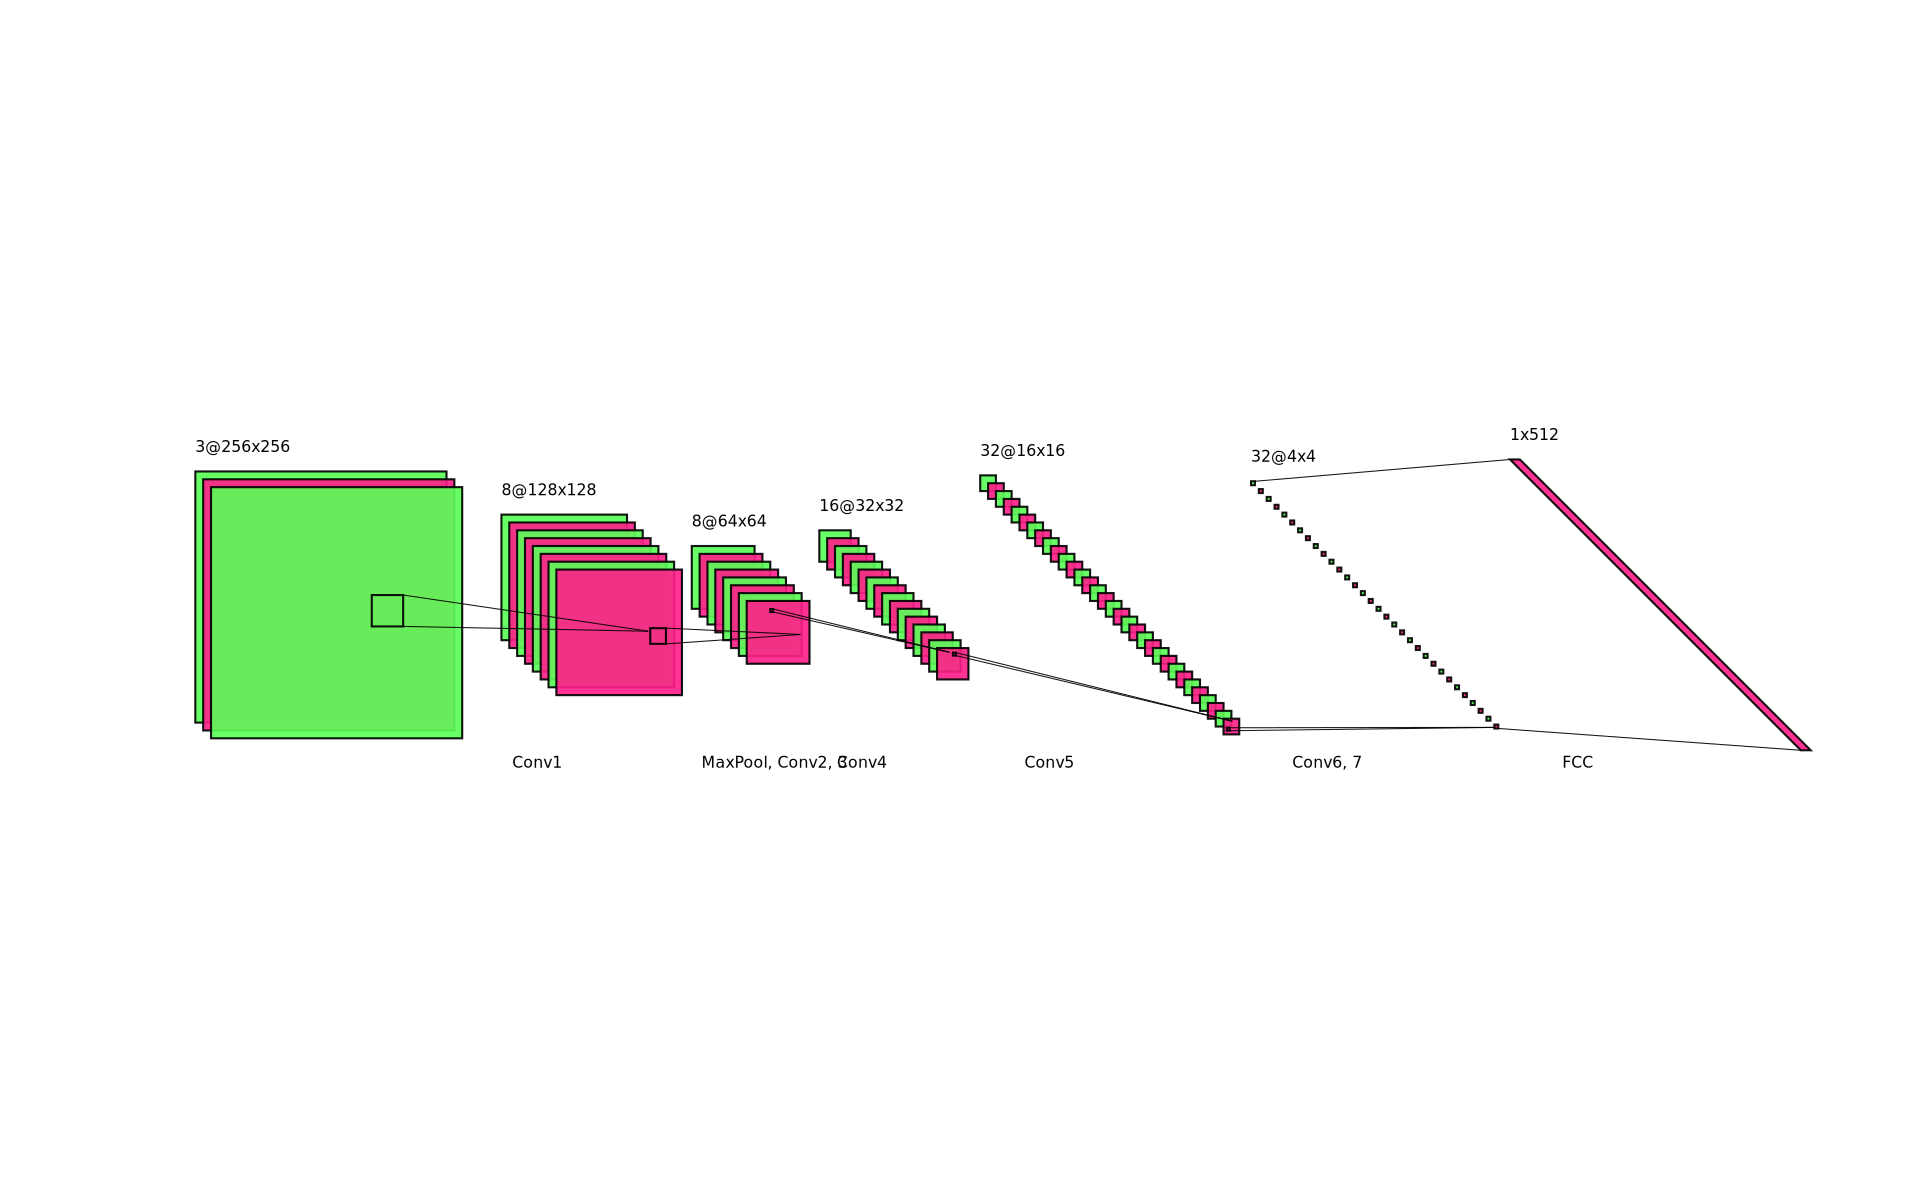
\includegraphics[scale=0.45]{figs/baseline.png}
    \end{center}
    \caption{Baseline model architecture, simplified; the final fully connected layer to a single output neuron.}
    \label{fig:baseline_arch}
\end{figure}

Across various hyperparameter combinations, we observed wide oscillations in our validation curves and overfitting. This is most likely due to the complex nature of the task, which demands greater parameters and epochs than ours. In our best model we were able to achieve a validation accuracy of 67.0\% and a testing accuracy of 65.6\%.

% \begin{table}[t]
%     \caption{Baseline model error statistics; real images are negatives and AI-generated images are positives.}
%     \label{baseline_stats}
%     \begin{center}
%         \begin{tabular}{llllll}
%             \multicolumn{1}{c}{\bf Split} & \multicolumn{1}{c}{\bf Loss} & \multicolumn{1}{c}{\bf Accuracy} & \multicolumn{1}{c}{\bf Precision} & \multicolumn{1}{c}{\bf Recall} & \multicolumn{1}{c}{\bf F1 Score}
%             \\ \hline \\
%             Training                      & 0.303                        & 87.3\%                           & 85.8\%                            & 89.5\%                         & 87.6\%                           \\
%             Validation                    & 0.947                        & 67.0\%                           & 66.2\%                            & 69.6\%                         & 67.8\%                           \\
%             Testing                       & 0.919                        & 65.6\%                           & 64.7\%                            & 68.5\%                         & 66.6\%                           \\
%         \end{tabular}
%     \end{center}
% \end{table}

% \begin{figure}[h]
%     \begin{center}
%         \includegraphics[scale=0.45]{figs/baseline_error_curves.png}
%         \includegraphics[scale=0.45]{figs/baseline_loss_curves.png}
%     \end{center}
%     \caption{Training/validation error (left) and loss (right) curves for the best baseline model.}
%     \label{fig:baseline_curves}
% \end{figure}

\section{Quantitative Results}
The EffVit Model achieved a final test accuracy of 85.9\% which is an essential indicator of success. The training and validation performance is shown in Figure \ref{fig:Gan_Conf}. As observed, the train and validation losses decrease almost simultaneously with roughly the same value throughout the 30 training epochs. Both loss begins to plateau around epoch 20 where the train and validation loss reaches 0.2938 and 0.2911 respectively at the end. The train and validation accuracies reaches 87.79\% and 87.29\% respectively. This suggests EffVit is learning the patterns of the embeddings of AI-generated images without over and underfitting. Detailed statistics of the model can be seen in Table \ref{tab:metrics} which will be further analyzed in section 9 Discussion.

\begin{figure}[h]
    \begin{center}
        \includegraphics[scale=0.27]{figs/training curves.png}
    \end{center}
    \caption{GAN-based models (CycleGAN, BigGAN, ProGAN) confidence levels}
    \label{fig:Training_Curves}
\end{figure}

\begin{table}[h]
    \centering
    \caption{Model Performance Metrics}
    \label{tab:metrics}
    \begin{tabular}{lcccc}
    \toprule
    \textbf{Metric} & \textbf{Test Accuracy} & \textbf{Precision} & \textbf{Recall} & \textbf{F1 Score} \\
    \midrule
    \textbf{Value}  & 85.9\%                & 86.1\%             & 85.56\%          & 85.8\%           \\
    \bottomrule
    \end{tabular}
    \end{table}
    


\section{Qualitative Results}
Quantitative results from the last section suggests decent performance of EffVit Model on determining AI-generated images. In the real world, fake images generated by a variety of architectures and models will observe contrasting high and low level features. To evaluate how well the model generalizes on images created by different models, six AI-generated images created by distinct models are selected from the test dataset. These images are then passed through the EffVit Model to obtain the output confidence levels.

It is observed that EffVit Model's confidence levels on images generated by GAN based models (CycleGAN, BigGAN, ProGAN) are relatively high according to Figure \ref{fig:Gan_Conf}. On the other hand, EffVit's confidence levels on images generated by Diffusion based models and transformer based models (GuidedDiffusion, Glide, Dalle-E Mini) are relatively low as shown in Figure \ref{fig:non-Gan_Conf}. EffVit may be learning subtle artifacts that images generated by GAN-based models have in common. This leads to high confidence on GAN generated images and lower confidence on images that don't contain those artifacts.

\begin{figure}[h]
    \begin{center}
        \includegraphics[scale=0.4]{figs/GAN_Confidence.png}
    \end{center}
    \caption{GAN-based models (CycleGAN, BigGAN, ProGAN) confidence levels}
    \label{fig:Gan_Conf}
\end{figure}
\begin{figure}[h]
    \begin{center}
        \includegraphics[scale=0.45]{figs/non-GAN_Confidence.png}
    \end{center}
    \caption{Non-GAN based models (GuidedDiffusion, Glide, Dalle-E Mini) confidence levels}
    \label{fig:non-Gan_Conf}
\end{figure}


\section{Performance on New Data}

\subsection{Data}

We evaluated our model on three sets of new data: real images from Caltech 256 \citep{griffinholubperona2022}, GAN-generated images from \citet{chuangchuangtanGANGenDetection}, and images generated by diffusion models from \citet{stable-diffusion-100k-custom-prompts-and-images}.

Caltech 256 was chosen for two reasons. First, there were enough images in the set that cropping to 224x224 would not remove too much of the image. Many other datasets with a range of semantics that we considered, for example Open Images \citep{Kuznetsova_2020}, do not contain images small enough for our model. Second, the images in Caltech 256 are very often edited. As shown in Figure \ref{fig:coco_vs_caltech}, many have their background removed, which marks a stark contrast from ImageNet and COCO, where objects are almost always in context. This is more representative of images on the internet, which are often edited, and allows us to evaluate our model for more general use.

\begin{figure}[h]
    \begin{center}
        \includegraphics[scale=0.3]{figs/coco_laptop.jpg}
        \includegraphics[scale=0.45]{figs/caltech_laptop.jpg}
    \end{center}
    \caption{Laptops in context, from COCO (left), and a laptop with its background removed, from Caltech 256 (right).}
    \label{fig:coco_vs_caltech}
\end{figure}

We used two datasets for AI-generated images because we wanted to evaluate the performance of our model on the two main types of architectures our model was trained on: GANs and diffusion models.

From these datasets, we used 984 real images, and $1,018$ fake images, selected at random.

\subsection{Evaluation}

On the new data, our model achieves an accuracy of 74.6\%. However, it is much better at identifying images generated by GANs than diffusion models. When only evaluating the GAN-generated dataset, its accuracy is 83.0\%, and when only evaluating the diffusion-model-generated dataset, its accuracy is 59.5\%. This is illustrated in the t-SNE of the hidden activations on the data shown in Figure \ref{fig:new_data_tsne}. We can see that the embeddings of most GAN-generated images form a cluster on the right, whereas most diffusion-model-generated image embeddings are spread throughout the large cluster of mostly real images on the left. However, there is a small cluster of diffusion-model-generated image embeddings at around $(25, -15)$, suggesting the model has learned something about this class of AI-generated images.

\begin{figure}[h]
    \begin{center}
        \includegraphics[width=0.6\textwidth]{figs/tsne.png}
    \end{center}
    \caption{t-SNE of final model's hidden activations on new dataset, by data type.}
    \label{fig:new_data_tsne}
\end{figure}

Due to the challenging nature of our data as described above, the achievement of our model exceeds our expectations. However, as mentioned in Section \ref{discussion}, we most likely could have improved our model's accuracy on images generated by diffusion models by using training data that was more balanced, relative to images generated by GANs.

\section{Discussion}
\label{discussion}


\section{Ethical Considerations}



\section{Project Difficulty}



\label{last_page}

\bibliography{APS360_ref}
\bibliographystyle{iclr2022_conference}

\end{document}
